\documentclass[dvipsnames, svgnames, leqno, a4paper, 12pt]{report}
\usepackage{preconfig}

\title{Teoria de Nevanlinna}
\date{}
\author{Daniel Benages}
\begin{document}
\shorthandoff{"}
    \maketitle
    \begin{abstract}
        WIP
    \end{abstract}
    \begin{chapter}{Introducció}
        L'objectiu d'aquest treball es donar un resultat sobre interpolació holomorfa dins el disc unitat, que denotarem per \(\D\). Per a això, començarem amb un breu estudi de les homografies. Aquestes ens permetran endinsar-nos en els automorfismes de \(\D\) i demostrar dos resultats de Schwarz i de Pick.

        Posteriorment parlarem de l'última peça clau: els productes de Blaschke finits. Finalment, amb tot l'arsenal disponible demostrarem el teorema de Pick-Nevanlinna:
        \begin{theorem*}[Pick-Nevanlinna]
            Siguin \(z_1,z_2,...,\) %enunciar bn el teorema 
        \end{theorem*}

        Aquesta tasca, però,  es inabordable sense fer algunes concessions. La més important es que donarem per fetes la majoria de nocions que s'obtindrien en un curs "elemental" d'anàlisi complexa, si més no, fins al teorema del mòdul màxim (tot i que l'enunciarem per refrescar la memòria). 
        
        Començarem amb unes definicions de conceptes bàsics, però que potser no s'arriben a veure habitualment.
        \begin{definition}[Funció Conforme] Sigui  \(\Omega\) un domini de \(\mathbb{C}\) i \(f: \Omega\to\Omega\) una funció holomorfa, diem que \(f\) és conforme si \(f'(z) \neq 0\,\  \forall z\in\Omega\).
        \end{definition}
        \begin{definition}[Esfera de Riemann]
            Diem esfera de Riemann a la compactificació del pla complex per un punt. La manera usual de pensar en aquest espai topològic és considerar una esfera on el pol nord es \(\infty\). La denotem per \(S^2\).
        \end{definition}
        No ens cal preocupar-nos per les propietats topològiques de \(S^2\), per al que a nosaltres ens ocupa, l'esfera de Riemann es comporta com \(\mathbb{C}\), però ens permet tractar \(\infty\) estalviant-nos limits. Es fàcil veure que \(1/0 = \infty\) i que \(1/\infty = 0\).

        De fet, aquest és el motiu principal per introduir el concepte de \(S^2\), ja que serveix de "cèrcol" per no deixar escapar els punts que habitualment hauríem de considerar pols de funcions altrament holomorfes. Per al nostre cas, ràpidament ens limitarem a no sortir de \(\D\).

    \end{chapter}
    \begin{chapter}{Homografies}
        \begin{definition}[Homografia]
            Siguin \(a,b,c,d\in S^2\). L'aplicació \begin{displaymath}
                z\to\frac{az+b}{cz+d}
            \end{displaymath}
            és una homografia.
        \end{definition}
        Observem que si \begin{math}
            z\neq -d/c
        \end{math}, les homografies són holomorfes a \begin{math}
            \mathbb{C}
        \end{math}
        \begin{proposition}
            Les homografies son invertibles i la seva inversa es una homografia.
        \end{proposition}
        \begin{proof}
            Si \begin{math}
                 w  = \frac{az+b}{cz+d} 
            \end{math}, podem aïllar $z$ i obtenim \begin{math}
                z = \frac{-d  w +b}{c w -a}
            \end{math}
        \end{proof}
        Es desprèn directament la següent proposició
        \begin{proposition}
            Les homografies son bijeccions de $S^2$.
        \end{proposition}
        Abans d'un teorema de caracterització veiem el següent lema:
        \begin{lemma}
            Donada $f$  una funció holomorfa tret d'un nombre finit de punts, si $f$ té un pol d'ordre igual o superior a 2, $f$ no pot ser injectiva.  
        \end{lemma}
        \begin{proof}
            Considerem la funció $1/f$. $f$ és injectiva si i només si $1/f$ ho és, per tant demostrar la no injectivitat de $1/f$ és suficient.
            
            Sigui $a$ un pol d'ordre $m>1$ de $f$. Llavors $a$ és un zero d'ordre $m$ de $1/f$, per tant \begin{math}
                \frac{1}{f}=(z-a)^mh(z)
            \end{math} amb $h(a)\neq0$, per a una certa funció holomorfa $h$.

            Considerem \begin{math}
                g(z)=(z-a)h(z)^{1/m}
            \end{math}. Aquesta funció és holomorfa i ben definida sobre l'arrel principal $m$-èssima. La seva derivada és 
            \begin{displaymath}
                g'(z)=\frac{1}{m}(z-a)h(z)^{\frac{1}{m}-1}h'(z)+h(z)^{\frac{1}{m}}
            \end{displaymath} per tant $g'(a)\neq0$.
            Tenim, doncs, un entorn de $a$ on $g$ és una funció holomorfa i invertible que envia $a$ al zero. Amb el canvi de coordenades $ w  = g(z)$, veiem que localment \begin{displaymath}
                 w ^m = \frac{1}{f(g^{-1}(z))}
            \end{displaymath} per tant en un entorn de $a$ la funció $1/f$ es comporta com la funció $z\to z^m$, que per $m>1$ no es injectiva.
        \end{proof}
        \begin{theorem}
            Si, tret d'un nombre finit de punts de $S^2$, tenim una bijecció conforme entre $S^2$ i una regió del propi $S^2$, aquesta bijecció es una homografia.
        \end{theorem}
        \begin{proof}
            Sigui $f$ aquesta bijecció i $q_1,\dots,q_n$ els punts exclòsos. Com $f$ és conforme, $f$ és holomorfa tret de en $q_i$. Aquests punts només poden ser pols, singularitats essencials o evitables. La possibilitat de que siguin essencials queda descartada, ja que en tot entorn d'una discontinuitat d'aquest tipus la imatge es tot el pla complex, per tant $f$ no podria ser bijectiva. Com les discontinuitats de $f$ són o evitables o pols, podem assegurar que $f$ es una funció racional. 
            
            A més, per la injectivitat a $S^2$, només un dels punts pot ser un pol, el qual pel lema anterior seria d'ordre 1. Si aquest es troba en un punt finit $q_k$, \begin{displaymath}
                f(z)=\frac{A_1}{z-q_k}+A_0=\frac{A_0z+A_1-A_0q_k}{z-q_k}\,\text{, } A_1\neq0
            \end{displaymath}
            Si $q_k=\infty$, \begin{displaymath}
                f(z)=A_1z+A_0\, \text{, } A_1\neq0
            \end{displaymath}
            Sigui com sigui, la funció és una homografia.
        \end{proof}
        \begin{proposition}\label{prop:comp_homo}
            La composició finita d'homografies és equivalent a una sola homografia.
        \end{proposition}
        \begin{proof}
            És suficient demostrar-ho per la composició de dues homografies. Siguin \begin{displaymath}
                T(z)=\frac{az+b}{cz+d}
            \end{displaymath}
            \begin{displaymath}
                S(z)=\frac{a'z+b'}{c'z+d'}
            \end{displaymath}
            Llavors\begin{displaymath}
                (T\circ S)(z)=\frac{a\frac{a'z+b'}{c'z+d'}+b}{c\frac{a'z+b'}{c'z+d'}+d}=\frac{aa'z+ab'+bc'z+bd'}{ca'z+cb'+dc'z+dd'}=\frac{\left( aa'+bc' \right)z+(ab'+bd')}{\left( ca'+dc' \right)z+(cb'+dd')}
            \end{displaymath}
            que clarament és una homografia.
        \end{proof}
        Degut a això, podem descomposar totes les homografies en combinacions de tres classes fonamentals:
        \begin{theorem}
            Tota homografia és composició finita de translacions, rotacions, homotècies i inversions.
        \end{theorem}
        \begin{proof}
            Totes aquestes transformacions són clarament homografies. Veiem que podem crear una cadena de composicions que ens porti a qualsevol homografia:
            
            Si $c=0$, simplement $z\to az\to az+b\to \frac{az+b}{d}$.

            Si $c\neq0$, llavors \begin{displaymath}
                z\to cz\to cz+d\to \frac{1}{cz+d}\to \frac{\frac{bc-ad}{c}}{cz+d}\to \frac{\frac{bc-ad}{c}}{cz+d}+\frac{a}{c}=\frac{bc-ad}{c(cz+d)}+\frac{a}{c}=\frac{bc-ad+azc+ad}{c(cz+d)}=\frac{az+b}{cz+d}
            \end{displaymath}
        \end{proof}
        \begin{definition}[Raó doble]
            Donats $z_1,z_2,z_3,z_4\in\mathbb{C}$, la raó doble entre ells es defineix per \begin{displaymath}
                (z_1,z_2,z_3,z_4) = \frac{(z_1-z_3)(z_2-z_4)}{(z_2-z_3)(z_1-z_4)}
            \end{displaymath}
            
            Ens serà útil considerar que algun d'aquests punts sigui $\infty$. En aquest cas, ometrem els termes que l'incloguin. Per exemple, si $z_1 = \infty$, llavors \begin{displaymath}
                (\infty, z_2,z_3,z_4) = \frac{z_2-z_4}{z_1-z_3}
            \end{displaymath}
        \end{definition}
    \begin{remark}
        Donats $z_1,z_2,z_3\in\mathbb{C}$, la funció donada per la raó doble \begin{equation}\label{eq:rao_doble}
            (z,z_1,z_2,z_3) = \frac{(z-z_2)(z_1-z_3)}{(z-z_3)(z_1-z_2)}=\frac{(z_1-z_3)z-z_2(z_1-z_3)}{(z_1-z_2)z-z_3(z_1-z_2)}
        \end{equation}
        és una homografia que envia $z_1\to1$, $z_2\to0$ i $z_3\to\infty$.

        A més, si algun $z_i$ és $\infty$, utilitzant la raó doble que pertoca es segueix complint aquesta afirmació.
    \end{remark}
    \begin{proposition}
        Les homografies conserven la raó doble.
    \end{proposition}
    \begin{proof}
        Siguin $z_1,z_2,z_3,z_4\in \C$ (finits), $z'_1,z'_2,z'_3,z'_4$ la seva imatge per una homografia que no envii cap a $\infty$.

        Tenim \begin{align*}
            z'_1-z'_3 &=\frac{az_1+b}{cz_1+d}-\frac{az_3+b}{cz_3+d} = \frac{acz_1z_3+adz_1+bcz_3+bd-acz_1z_3-adz_3-bcz_1-bd}{(cz_1+d)(cz_3+d)} = \\
            &= \frac{(ad-bc)(z_1-z_3)}{(cz_1+d)(cz_3+d)}
        \end{align*}
        Ídem per a $z'_1-z'_4, z'_2-z'_4, z'_2-z'_3$, per tant un cop simplifiquem tenim 
        \begin{displaymath}
            \frac{(z'_1-z'_3)(z'_2-z'_4)}{(z'_1-z'_4)(z'_2-z'_3)}=\frac{\frac{(ad-bc)^2(z_1-z_3)(z_2-z_4)}{(cz_1+d)(cz_2+d)(cz_3+d)(cz_4+d)}}{\frac{(ad-bc)^2(z_1-z_4)(z_2-z_3))}{(cz_1+d)(cz_2+d)(cz_3+d)(cz_4+d)}} = \frac{(z_1-z_3)(z_3-z_4)}{(z_1-z_4)(z_2-z_3)}
        \end{displaymath}
        Per ultim, suposem un dels punts es $\infty$. Per exemple, sigui $z'_1=\infty$, tenim que $d=-cz_1$. La raó doble de les imatges és \begin{displaymath}
            (\infty,z'_2,z'_3,z'_4)=\frac{(z'_2-z'_4)}{(z'_2-z'_3)}=\frac{(z_2-z_4)(cz_3+d)}{(z_2-z_3)(cz_4+d)}=\frac{(z_2-z_4)(cz_3-cz_1)}{(z_2-z_3)(cz_4-cz_1)}=\frac{(z_1-z_3)(z_2-z_4)}{(z_1-z_4)(z_2-z_3)}
        \end{displaymath}
    \end{proof}
    \begin{theorem}
        La única homografia que deixa fixos més de dos punts és la identitat.
    \end{theorem}
    \begin{proof}
        Donada la homografia $\frac{az+b}{cz+d}$, els seus punts fixos compleixen \begin{displaymath}
            \frac{az+b}{cz+d}=z\implies cz^2+(d-a)z+b=0
        \end{displaymath}
        Si $c=0$, només hi ha un punt fix $z=\frac{b}{d-a}$.

        Si $c\neq0$, tenim una equació de segon grau i l'única forma que es compleixi per a tot $z$ es que $c=b=0$ i $a=d$, per tant \begin{displaymath}
            \frac{az+b}{cz+d}=\frac{az}{a}=z\implies \text{és la aplicació identitat.}
        \end{displaymath}
    \end{proof}
    Això ens porta al teorema de caracterització de les homografies.
    \begin{theorem}
        Tota homografia està definida per les imatges de tres punts diferents. 

        És a dir, donats $z_1,z_2,z_3,z_4,z'_1,z'_2,z'_3,z'_4\in\C$, existeix una única homografia $T$ tal que $T(z_1)=z'_1$, $T(z_2)=z'_2$, $T(z_3)=z'_3$, $T(z_4)=z'_4$.
    \end{theorem}
    \begin{proof}
        Demostrem primer la unicitat. Siguin $S$, $T$ dues homografies tals que $S(z_i)=T(z_i)=z'_i$. Llavors $S^{-1}T$ és una homografia per Proposició \ref{prop:comp_homo} que compleix \[S^{-1}T(z_i)=S^{-1}(z'_i)=z_i\, i=1,\dots4\]. Com té quatre punts fixos, $S^{-1}T=id\implies T=S$.

        Per veure l'existència, recordem que per (\ref{eq:rao_doble}), la rao doble $(z,z_1,z_2,z_3)$ ens envia $z_1\to1,\, z_2\to0,\, z_3\to\infty$. 
        Siguin $S=(z,z'_1,z'_2,z'_3)$ i $T=(z,z_1,z_2,z_3)$
        Llavors, la composició \begin{displaymath}
            S^{-1}\circ T
        \end{displaymath}
        és la homografia que busquem.
    \end{proof}
\end{chapter}
\begin{chapter}[Automorfismes al Disc Unitat]{Automorfismes a $\D$}
    Com ja hem comentat prèviament, centrarem la nostra atenció exclusivament a $\D$, per tant els teoremes i proposicions que enunciarem a partir d'ara seran sempre en aquesta regió. Recordem primer la definició \begin{definition}{Disc Unitat $\D$}
        Definim la regió de $\C$ anomenada Disc Unitat com \begin{equation}
            \D=\{\, z\in\C\mid |z|<1\, \}
        \end{equation}
    \end{definition}
    \begin{remark}
        La regió $\D$ és un domini acotat de $\C$.
    \end{remark}

    Enunciem ara el Teorema del Mòdul Màxim que, tot i que no el demostrarem (ens portaria massa feina i ens allunyaria de l'objectiu del treball), ens serà indispensable per als propers resultats. 
    \begin{theorem}[Teorema del Mòdul Màxim]\label{th:TMM}
        Sigui $K$ la clausura d'una regió acotada $\Omega$. Si $f$ és continua en $K$ i holomorfa en $\Omega$, llavors \begin{equation}
            \abs{f(z)}\leq\norm{f}_{\partial\Omega},\;\forall z\in\Omega.
        \end{equation}
        Si es dona la igualtat per a algun $z\in\Omega$, llavors $f$ és constant.
    \end{theorem}
    Enunciem ara el Teorema de caracterització dels automorfismes holomorfs de $\D$:
    \begin{theorem}
        Una funció $T:\D\to\D$ holomorfa és bijectiva si i només si \begin{equation}
            T(z)=\lambda\frac{a-z}{1-\overline{a}z},\, \text{amb }a\in\D\; \text{ i }\; \abs{\lambda}=1.
        \end{equation}
    \end{theorem}
    Dit d'una altra manera, els automorfismes del disc són una classe molt concreta d'homografies.
    \begin{proof}
        Pel que ja hem vist, sabem que $T(z)=\lambda\frac{a-z}{1-\overline{a}z}$ és automorfisme holomorf de $\C$. Només cal veure que és bijectiu a $\D$. 

        Sigui $z\in\D$. Tenim\begin{align}
            \frac{\abs{a-z}}{\abs{1-\overline{a}z}}<1 &\iff \abs{a-z}^2<\abs{1-\overline{a}z}^2\iff\abs{a}^2+\abs{z}^2-2\Re{a\overline{z}}<1+\abs{\overline{a}z}^2-2\Re{\overline{\overline{a}z}}\iff\\
            &\iff\abs{a}^2\abs{z}^2-\abs{a}^2\abs{z}^2-1<0\iff\left( \abs{z}^2-1 \right)\left( 1-\abs{a}^2 \right)<0\iff\abs{a}<1
        \end{align}
        Per tant $\D\xrightarrow{T} \D$ és automorfisme holomorf.

        Vegem ara la implicació contraria. Sigui $T:\D\to\D$ holomorfa i bijectiva. 
        Suposem primer que $T(0)=0$. Com $T$ és holomorfa, és una serie de potencies i si deixa el 0 fix, $\frac{T(z)}{z}$ és holomorfa en $\D$. Considerem $\abs{\frac{T(z)}{z}}$ en un disc $U$ de radi $r<1$ centrat a l'origen. Pel Teorema del Mòdul Màxim \ref{th:TMM}, $T(z)/z$ és màxim en $\abs{z}=r$. Llavors en $U$ tenim \begin{displaymath}
            \abs{\frac{T(z)}{z}}<\frac{1}{r}\xrightarrow{r\to1}\abs{\frac{T(z)}{z}}\leq1,\, \text{en }\D
        \end{displaymath}
        Sigui $S$ la inversa de $T$, pel mateix raonament tenim $\abs{\frac{S(z)}{z}}<1$ en $\D$. Així doncs\begin{displaymath}
            \frac{S(z)}{z}=\frac{z}{T(z)}\implies \abs{\frac{T(z)}{z}}=1,\; \forall z\in\D.
        \end{displaymath}
        i com el valor absolut es constant, també ho és la funció (pel fet de ser holomorfa), llavors \begin{equation}
            \frac{T(z)}{z}=e^{i\alpha}\implies T(z)=e^{i\alpha}z
        \end{equation}
        per una $\alpha\in\mathbb{R}$ constant. Per tant, un automorfisme bijectiu de $\D$ que fixa l'origen és una rotació. 

        Eliminem la restricció de que l'origen sigui fix. Sigui $T(z)=a\neq0$. Considerem l'homografia \begin{displaymath}
            R=\lambda\frac{a-z}{1-\overline{a}z}
        \end{displaymath}
        amb $\lambda=e^{i\beta}$, $\beta\in\mathbb{R}$. La composició $R^{-1}T$ és un automorfisme holomorf de $\D$ que deixa fix l'origen, per tant és una rotació, diguem $e^{i\alpha}$. 

        Llavors \begin{displaymath}
            R^{-1}T=e^{i\alpha}\implies T=Re^{i\alpha}\implies T(z)=e^{i(\alpha+\beta)}\frac{a-z}{1-\overline{a}z}=\lambda'\frac{a-z}{1-\overline{a}z}
        \end{displaymath}
    \end{proof}
    
    A partir d'ara, denotarem \begin{equation}
        \varphi_a(z):=\frac{a-z}{1-\overline{a}z}
    \end{equation}
    Vegem ara un clàssic de l'anàlisi complexa
    \begin{theorem}[Lema de Schwarz]\label{th:sch}
        Sigui $f:\D\to\D$ una funció holomorfa amb $f(0)=0$.

        Aleshores
        \begin{enumerate}[(i)]
            \item $\abs{f(z)}\leq\abs{z}$ per a tot $z\in\D$
            \item $\abs{f'(0)}\leq 1$
        \end{enumerate}
        A més, si hi hagués igualtat en algun dels dos casos, aleshores $f(z)=e^{i\alpha}z$ per a algun $\alpha\in\mathbb{R}$ i per a tot $z\in\D$.
    \end{theorem} 
    \begin{proof}
        Demostrarem primer \textit{(i)}.

        Com $f(0)=0$ i és holomorfa, tenim que $h(z)=f(z)/z$ és holomorfa en tot $\D$. Pel Teorema del mòdul màxim \ref{th:TMM}, \begin{equation}
            \sup_{\abs{z}\leq r}\abs{h(z)}=\sup_{\abs{z}= r}\abs{h(z)}=\frac{1}{r}\sup_{\abs{z}\leq r}\abs{f(z)}
        \end{equation}
        per a $0<r<1$. Com $\abs{f(z)}\leq 1$ per a tot $z\in\D$, fem tendir $r$ a 1 i tenim \begin{equation}
            \sup_{z\in\D}\abs{h(z)}\leq 1\implies \abs{f(z)}\leq \abs{z}
        \end{equation}
        Veiem a més que si $\abs{f(z_0)}=\abs{z_0}$ per a algun $z_0\in\D\setminus\{0\}$, llavors $\abs{h(z_0)}=1$ i pel teorema del mòdul màxim, $h$ és constant de mòdul 1, és a dir, $\exists\alpha\in\mathbb{R}$ tal que \begin{displaymath}
            f(z)=zh(z)=ze^{i\alpha}, \; \forall z\in\D.
        \end{displaymath}
        
        Vegem ara \textit{(ii)}.

        Com $f(z)/z=h(z)$ i $f(0)=0$, llavors \begin{equation}
            \abs{f'(0)}=\lim_{z\to0}\frac{\abs{f(z)}}{\abs{z}}=\lim_{z\to0}\abs{h(z)}=\abs{h(0)}\leq1
        \end{equation} 
        A més, si $\abs{f'(0)}=\abs{h(0)}=1$, pel teorema del mòdul màxim un altre cop tenim $h=e^{i\alpha}$ per a un cert $\alpha\in\mathbb{R}$ i per tant $f(z)=e^{i\alpha}z$, $\forall z\in\D$.
    \end{proof}

    No tan famosa és una generalització d'aquest lema, on es relaxen les hipòtesis i no es suposa que $f(0)=0$. Aquest és el lema de Schwarz-Pick:
    \begin{theorem}[Lema de Schwarz-Pick]\label{lema:SP}
        Sigui $f:\D\to\D$ una funció holomorfa. Llavors
        \begin{enumerate}[(i)]
            \item \(\displaystyle \abs{\frac{f(z)-f( w )}{1-f(z)\overline{f( w )}}}\leq\frac{z- w }{1-z\overline{ w }},\text{ per a tot }z, w \in\D\)
            \item \(\displaystyle \frac{\abs{f'(z)}}{1-\abs{f(z)}^2}\leq\frac{1}{1-\abs{z}^2}\text{ per a tot }z\in\D\) 
        \end{enumerate}
        La igualtat en tots dos casos es dona si $f$ és automorfisme de $\D$.

        Si la igualtat de \textit{(i)} es compleix per $z\neq w $, o si es compleix \textit{(ii)} en un $z$, llavors $f$ és automorfisme de $\D$.
    \end{theorem} 
    \begin{proof}
        Sigui $g = \varphi_{f( w )}\circ f\circ \varphi_{- w }$. $g$ és un automorfisme de $\D$ holomorf. 
        \begin{sloppypar}Com \({\displaystyle g(z)=\varphi_{f( w )}\left( f\left( \frac{z+ w }{1+\overline{ w }z} \right) \right)}\), en particular tenim $g(0)=\varphi_{f( w )}\left( f( w ) \right)=0$. Pel lema de Schwarz \ref{th:sch}, $\abs{g(\xi)}\leq\abs{\xi}$ per a tot $\xi\in\D$ i \begin{displaymath}
            \abs{g(\varphi_{f( w )}(z))}\leq\abs{\varphi_{ w }(z)}\implies\abs{\varphi_{f( w )}(f(z))}\leq\abs{\varphi_ w (z)}
        \end{displaymath} i substituint cada terme per la seva definició \begin{equation}
            \abs{\frac{f(z)-f( w )}{1-\overline{f( w )}f(z)}}\leq\abs{\frac{z- w }{1-\overline{ w }z}}
        \end{equation}\end{sloppypar}
        Si tenim igualtat per uns $z\neq w $, llavors $\abs{g(\varphi_ w (z))}=\abs{\varphi_ w (z)}$ i pel lema de Schwarz, $g(z)=ze^{i\alpha}\implies g$ és un automorfisme de $\D\implies$ $f=\varphi_{-f( w )}\circ g\circ \varphi_ w $ també.
        Veiem ara \textit{(ii)}.

        \begin{displaymath}
            \frac{\abs{f'(z)}}{1-\abs{f(z)}^2}=\lim_{ w \to z}\left( \abs{\frac{f(z)-f( w )}{z- w }}\frac{1}{\abs{1-\overline{f( w )}f(z)}} \right)\leq\lim_{ w \to z}\frac{1}{1-\overline{ w }z}=\frac{1}{1-\abs{z}^2}
        \end{displaymath}

        Si tenim igualtat a \textit{(ii)}, considerem $z= w $ i com \(\displaystyle \varphi_{a}'(z)=\frac{1-\abs{a}^2}{(1-\overline{a}z)^2}\), tenim \begin{align*}
            \abs{g'(0)} &= \abs{\varphi_{f( w )}'(f\circ\varphi_{- w }'(0))}\abs{f'\left( \varphi_{- w }(0) \right)}\abs{\varphi_{- w }'(0)}=\\
            &=\abs{\varphi_{f( w )}'\left( f( w ) \right)}\abs{f'( w )}\left( 1-\abs{ w }^2 \right)=\\
            &=\frac{1-\abs{f( w )}^2}{\left( 1-\overline{f( w )}f( w ) \right)^2}\abs{f'( w )}\left( 1-\abs{ w }^2 \right)=\\
            &=\frac{\abs{f'( w )}}{1-\abs{f( w )}^2}\left( 1-\abs{ w }^2 \right)=1
        \end{align*}
        i, pel Lema de Schwarz, $g$ és automorfisme i $f=\varphi_{-f( w )}\circ g\circ \varphi_ w $ també. 

        Finalment, si $f$ és automorfisme de $\D$, apliquem \textit{(i)} a $f$ i $f^{-1}$ i obtenim \begin{equation}
            \abs{\frac{z- w }{1-z\overline{ w }}}=\abs{\frac{f^{-1}(f(z))-f^{-1}(f( w ))}{1-f^{-1}(f(z))\overline{f^{-1}(f( w ))}}}\leq\abs{\frac{f(z)-f( w )}{1-f(z)\overline{f( w )}}}\leq\abs{\frac{z- w }{1-z\overline{ w }}}
        \end{equation} per tant igualtat.
        De la mateixa manera, per a \textit{(ii)} tenim \begin{equation}
            \frac{1}{1-\abs{z}^2}=\frac{\abs{(f^{-1}\circ f)'(z)}}{1-\abs{(f^{-1}\circ f)(z)}^2}\leq\frac{f'(z)}{1-\abs{f(z)}^2}\leq\frac{1}{1-\abs{z}^2}
        \end{equation} per tant igualtat.
    \end{proof}
\end{chapter}
\chapter{El Teorema de Pick}
L'última peça clau per al problema d'interpolació són els productes de Blaschke. No ens caldrà anar més enllà del cas finit.

Un \textbf{producte de Blaschke finit} és una funció de la forma \begin{displaymath}
    B(z)=e^{i\alpha}\prod_{j=1}^{n}\frac{z-z_j}{1-\overline{z_j}z},\;\ \abs{z_j}<1
\end{displaymath}
Ens seran útils les següents propietats
\begin{proposition}
    Si $B$ és un producte de Blaschke és compleix:
    \begin{enumerate}[(i)]
        \item $B$ és continua en $\partial\D$
        \item $\abs{B}=1$ en $\partial\D$
        \item $B$ té un nombre finit de zeros en $\D$
    \end{enumerate}
    Aquestes propietats, junt amb on són aquestes zeros, determinen $B$ tret d'una constant de mòdul 1.
\end{proposition}
\begin{proof}
    No demostrarem $(i)$, $(ii)$, $(iii)$; el que demostrarem és això últim.

    Si tenim una funció $f$ que compleix les tres i $B$ un producte de Blaschke amb els mateixos zeros, pel principi del mòdul màxim, $\abs{f/B}\leq1$ i $\abs{B/f}\leq1$ en $\D$. Per tant $f/B$ és constant.
\end{proof}
Els productes de Blaschke, a més de ser útils en la interpolació (com veurem pròximament),  juguen un paper important en l'aproximació de funcions del disc. 
\begin{theorem}{Carathéodory}
    Sigui $f$ un $\D$-holomorfisme. Existeix $\{B_k\}$ una successió de productes de Blaschke que convergeixen puntualment a $f$.
\end{theorem}
\begin{proof}
    Com $f$ és holomorfa, és una serie de potencies. Siguin $\{c_k\}$ els seus coeficients. Demostrarem el teorema per inducció, trobant un producte de Blaschke de grau com a molt $n$ tal que els $n$ primers coeficients coincideixen amb els de $f$, i.e., \begin{displaymath}
        B_n=c_0+c_1z+\dots+c_{n-1}z^{n-1}+d_nz^n\dots
    \end{displaymath}
    Com $\abs{c_0}\leq1$, podem fixar $B_0=\frac{z+c_0}{1+\overline{c_0}z}$. Si $\abs{c_0}=1$, llavors $B_0=c_0$ és un producte de Blaschke de grau 0.

    Suposem que per a qualsevol $g$ $\D$-holomorfisme tenim construït el seu $B_{n-1}/z)$. Sigui $g=\frac{1}{z}\frac{f-f(0)}{1-\overline{f(0)}f}$ i sigui $B_{n-1}(z)$ el producte de Blaschke de grau com a màxim $n-1$ tal que $g-B_{n-1}$ té un zero d'ordre $n-1$ en $z=0$. Llavors $zg-zB_{n-1}$ té un zero d'ordre $n$ en $0$. 
    
    Sigui \begin{displaymath}
        B_n(z)= \frac{zB_{n-1}+f(0)}{1+\overline{f(0)}zB_{n-1}(z)}
    \end{displaymath}
    Llavors $B_n(z)$ és un producte de Blaschke, $\text{grau}(B_n)=\text{grau}(zB_{n-1})\leq n$ i 
    \footnotesize
    \begin{displaymath}
        f(z)-B_n(z)=\frac{zg(z)+f(0)}{1+\overline{f(0)}zg(z)}-\frac{zB_{n-1](z)+f(0)}}{1+\overline{f(0)}zB_{n-1}(z)}=\frac{(1-\abs{f(0)}^2z(g(z)-B_{n-1}(z)))}{(1+\overline{f(0)}zg(z))(1+\overline{f(0)}zB_{n-1}(z))}
    \end{displaymath}
    \normalsize
    per tant $f-B_n$ té un zero d'ordre $n$ en $z=0$ i llavors \begin{displaymath}
        B_n(z)=c_0+c_1z+\dots+c_nz^n+d_{n+1}z^{n+1}
    \end{displaymath}
\end{proof}
Per últim, un lema que ens ajudarà amb la demostració del Teorema de Pick

\begin{lemma}
    Siguin $z_1. z_2\in\D$ diferents i siguin $ w _1, w _2\in\C$. Les següents afirmacions són equivalents:
    \begin{enumerate}[(i)]
        \item Existeix $f$ un $\D$-holomorfisme tal que $f(z_1)=w_1$, $f(z_2)=w_2$.
        \item La forma quadràtica \(\displaystyle Q_2(t_1,t_2)=\sum_{j,k=1}^2\frac{1-w_j\overline{w_k}}{1-z_j\overline{z_k}}t_j\overline{t_k}\leq0\)
        \item \(\displaystyle \abs{\frac{w_2-w_1}{1-\overline{w_1}w_2}}\leq\abs{\frac{z_2-z_1}{1-\overline{z_1}z_2}}\)
        \item \(\displaystyle \frac{(1-\abs{w_2}^2)(1-\abs{w_1}^2)}{\abs{1-\overline{w_1}w_2}^2}\geq\frac{(1-\abs{z_1}^2)(1-\abs{z_2}^2)}{\abs{1-\overline{z_1}z_2}^2}\)
    \end{enumerate}
\end{lemma}
    \begin{proof} Veurem $(i)\iff(iii)\iff(iv)\iff(ii)$

        \large
        $(i)\implies(iii)$
        \normalsize
        És el Lema de Schwarz-Pick \ref{lema:SP}.
        
        \large
        $(iii)\implies(i)$
        \normalsize
        Construïm $f=\tau_3^{-1}\circ\tau_2\circ\tau_1$ a partir de la figura (\ref{fig:lema-prev-pick}).

\begin{figure}[H]
    \centering
    \tikzset{every picture/.style={line width=0.75pt}} %set default line width to 0.75pt        

    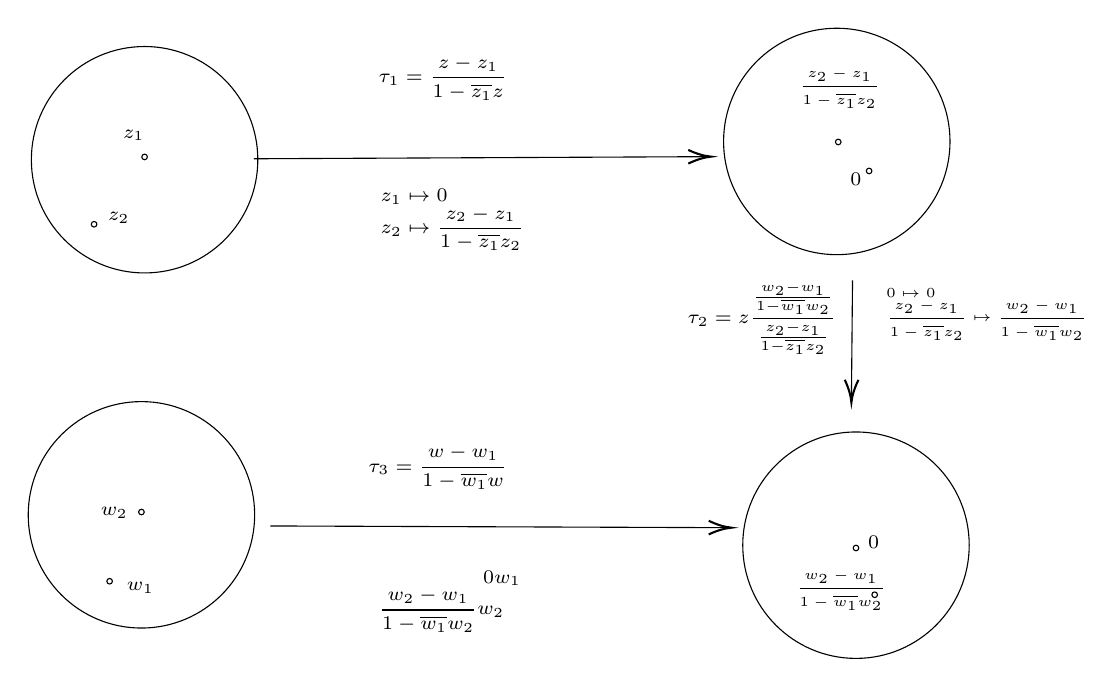
\begin{tikzpicture}[x=0.75pt,y=0.75pt,yscale=-1,xscale=1]
    %uncomment if require: \path (0,407); %set diagram left start at 0, and has height of 407
    
    %Shape: Ellipse [id:dp1940871183710945] 
    \draw   (355.2,82.55) .. controls (355.2,52.42) and (379.62,28) .. (409.74,28) .. controls (439.87,28) and (464.29,52.42) .. (464.29,82.55) .. controls (464.29,112.67) and (439.87,137.1) .. (409.74,137.1) .. controls (379.62,137.1) and (355.2,112.67) .. (355.2,82.55) -- cycle ;
    %Shape: Ellipse [id:dp46982186242036084] 
    \draw   (74.89,90) .. controls (74.89,89.26) and (75.49,88.65) .. (76.24,88.65) .. controls (76.99,88.65) and (77.59,89.26) .. (77.59,90) .. controls (77.59,90.75) and (76.99,91.36) .. (76.24,91.36) .. controls (75.49,91.36) and (74.89,90.75) .. (74.89,90) -- cycle ;
    %Shape: Circle [id:dp8460884941367898] 
    \draw   (50.55,122.45) .. controls (50.55,121.7) and (51.16,121.1) .. (51.91,121.1) .. controls (52.65,121.1) and (53.26,121.7) .. (53.26,122.45) .. controls (53.26,123.2) and (52.65,123.8) .. (51.91,123.8) .. controls (51.16,123.8) and (50.55,123.2) .. (50.55,122.45) -- cycle ;
    %Shape: Circle [id:dp22422351868171242] 
    \draw   (423.96,96.76) .. controls (423.96,96.02) and (424.57,95.41) .. (425.31,95.41) .. controls (426.06,95.41) and (426.66,96.02) .. (426.66,96.76) .. controls (426.66,97.51) and (426.06,98.12) .. (425.31,98.12) .. controls (424.57,98.12) and (423.96,97.51) .. (423.96,96.76) -- cycle ;
    %Shape: Ellipse [id:dp05578671192736695] 
    \draw   (409.09,82.79) .. controls (409.09,82.05) and (409.69,81.44) .. (410.44,81.44) .. controls (411.19,81.44) and (411.79,82.05) .. (411.79,82.79) .. controls (411.79,83.54) and (411.19,84.15) .. (410.44,84.15) .. controls (409.69,84.15) and (409.09,83.54) .. (409.09,82.79) -- cycle ;
    %Shape: Ellipse [id:dp7086048713327018] 
    \draw   (417.64,278.41) .. controls (417.64,277.67) and (418.24,277.06) .. (418.99,277.06) .. controls (419.74,277.06) and (420.34,277.67) .. (420.34,278.41) .. controls (420.34,279.16) and (419.74,279.76) .. (418.99,279.76) .. controls (418.24,279.76) and (417.64,279.16) .. (417.64,278.41) -- cycle ;
    %Shape: Ellipse [id:dp8993168803355189] 
    \draw   (426.65,300.94) .. controls (426.65,300.2) and (427.26,299.59) .. (428,299.59) .. controls (428.75,299.59) and (429.35,300.2) .. (429.35,300.94) .. controls (429.35,301.69) and (428.75,302.3) .. (428,302.3) .. controls (427.26,302.3) and (426.65,301.69) .. (426.65,300.94) -- cycle ;
    %Shape: Ellipse [id:dp7992364884312477] 
    \draw   (73.37,261.09) .. controls (73.37,260.34) and (73.98,259.74) .. (74.72,259.74) .. controls (75.47,259.74) and (76.08,260.34) .. (76.08,261.09) .. controls (76.08,261.84) and (75.47,262.44) .. (74.72,262.44) .. controls (73.98,262.44) and (73.37,261.84) .. (73.37,261.09) -- cycle ;
    %Shape: Ellipse [id:dp09061757542467885] 
    \draw   (58.05,294.44) .. controls (58.05,293.69) and (58.66,293.09) .. (59.4,293.09) .. controls (60.15,293.09) and (60.75,293.69) .. (60.75,294.44) .. controls (60.75,295.18) and (60.15,295.79) .. (59.4,295.79) .. controls (58.66,295.79) and (58.05,295.18) .. (58.05,294.44) -- cycle ;
    %Shape: Ellipse [id:dp5032465020293418] 
    \draw   (21.69,91.36) .. controls (21.69,61.23) and (46.11,36.81) .. (76.24,36.81) .. controls (106.37,36.81) and (130.79,61.23) .. (130.79,91.36) .. controls (130.79,121.48) and (106.37,145.9) .. (76.24,145.9) .. controls (46.11,145.9) and (21.69,121.48) .. (21.69,91.36) -- cycle ;
    %Shape: Ellipse [id:dp6875011805442678] 
    \draw   (364.44,277.06) .. controls (364.44,246.93) and (388.86,222.51) .. (418.99,222.51) .. controls (449.12,222.51) and (473.54,246.93) .. (473.54,277.06) .. controls (473.54,307.19) and (449.12,331.61) .. (418.99,331.61) .. controls (388.86,331.61) and (364.44,307.19) .. (364.44,277.06) -- cycle ;
    %Shape: Ellipse [id:dp3952214457400949] 
    \draw   (20.18,262.44) .. controls (20.18,232.32) and (44.6,207.89) .. (74.72,207.89) .. controls (104.85,207.89) and (129.27,232.32) .. (129.27,262.44) .. controls (129.27,292.57) and (104.85,316.99) .. (74.72,316.99) .. controls (44.6,316.99) and (20.18,292.57) .. (20.18,262.44) -- cycle ;
    
    % Text Node
    \draw (114.92,82.43) node [anchor=north west][inner sep=0.75pt]   [align=left] {};
    % Text Node
    \draw (352.13,81.34) node [anchor=north west][inner sep=0.75pt]   [align=left] {};
    % Text Node
    \draw (187.72,40.4) node [anchor=north west][inner sep=0.75pt]  [font=\scriptsize] [align=left] {$\displaystyle \tau _{1} =\frac{z-z_{1}}{1-\overline{z_{1}} z}$};
    % Text Node
    \draw (188.72,104.29) node [anchor=north west][inner sep=0.75pt]  [font=\scriptsize] [align=left] {$\displaystyle z_{1} \mapsto 0$\\$\displaystyle z_{2} \mapsto \frac{z_{2} -z_{1}}{1-\overline{z_{1}} z_{2}}$};
    % Text Node
    \draw (411.95,128.43) node [anchor=north west][inner sep=0.75pt]   [align=left] {};
    % Text Node
    \draw (411.16,212.34) node [anchor=north west][inner sep=0.75pt]   [align=left] {};
    % Text Node
    \draw (336.6,149.14) node [anchor=north west][inner sep=0.75pt]  [font=\scriptsize] [align=left] {$\displaystyle \tau _{2} =z\frac{\frac{w_{2} -w_{1}}{1-\overline{w_{1}} w_{2}}}{\frac{z_{2} -z_{1}}{1-\overline{z_{1}} z_{2}}}$};
    % Text Node
    \draw (432.4,151.98) node [anchor=north west][inner sep=0.75pt]  [font=\tiny] [align=left] {$\displaystyle 0\mapsto 0$\\$\displaystyle \frac{z_{2} -z_{1}}{1-\overline{z_{1}} z_{2}} \mapsto \frac{w_{2} -w_{1}}{1-\overline{w_{1}} w_{2}}$};
    % Text Node
    \draw (122.89,259.27) node [anchor=north east][inner sep=0.75pt]  [xscale=-1] [align=left] {};
    % Text Node
    \draw (361.97,260.17) node [anchor=north east][inner sep=0.75pt]  [xscale=-1] [align=left] {};
    % Text Node
    \draw (182.78,227.99) node [anchor=north west][inner sep=0.75pt]  [font=\scriptsize] [align=left] {$\displaystyle \tau _{3} =\frac{w-w_{1}}{1-\overline{w_{1}} w}$};
    % Text Node
    \draw (187.78,288.09) node [anchor=north west][inner sep=0.75pt]  [font=\scriptsize] [align=left] {$\displaystyle \ \ \ \ \ \ \ \ \ \ \ \ \ \ 0\mapsfrom w_{1}$\\$\displaystyle \frac{w_{2} -w_{1}}{1-\overline{w_{1}} w_{2}} \mapsfrom w_{2}$};
    % Text Node
    \draw (64.61,75.67) node [anchor=north west][inner sep=0.75pt]  [font=\scriptsize] [align=left] {$\displaystyle z_{1}$};
    % Text Node
    \draw (57.4,115.32) node [anchor=north west][inner sep=0.75pt]  [font=\scriptsize] [align=left] {$\displaystyle z_{2}$};
    % Text Node
    \draw (390.44,45.85) node [anchor=north west][inner sep=0.75pt]  [font=\tiny] [align=left] {$\displaystyle \frac{z_{2} -z_{1}}{1-\overline{z_{1}} z_{2}}$};
    % Text Node
    \draw (415.08,96.45) node [anchor=north west][inner sep=0.75pt]  [font=\scriptsize] [align=left] {0};
    % Text Node
    \draw (423.63,271.34) node [anchor=north west][inner sep=0.75pt]  [font=\scriptsize] [align=left] {0};
    % Text Node
    \draw (389,287.82) node [anchor=north west][inner sep=0.75pt]  [font=\fontsize{0.47em}{0.56em}\selectfont] [align=left] {$\displaystyle \frac{w_{2} -w_{1}}{1-\overline{w_{1}} w_{2}}$};
    % Text Node
    \draw (66.5,293.62) node [anchor=north west][inner sep=0.75pt]  [font=\scriptsize] [align=left] {$\displaystyle w_{1}$};
    % Text Node
    \draw (53.88,257.57) node [anchor=north west][inner sep=0.75pt]  [font=\scriptsize] [align=left] {$\displaystyle w_{2}$};
    % Connection
    \draw    (128.92,90.89) -- (347.13,89.88) ;
    \draw [shift={(349.13,89.87)}, rotate = 539.73] [color={rgb, 255:red, 0; green, 0; blue, 0 }  ][line width=0.75]    (10.93,-3.29) .. controls (6.95,-1.4) and (3.31,-0.3) .. (0,0) .. controls (3.31,0.3) and (6.95,1.4) .. (10.93,3.29)   ;
    % Connection
    \draw    (417.33,149.43) -- (416.79,206.34) ;
    \draw [shift={(416.78,208.34)}, rotate = 270.54] [color={rgb, 255:red, 0; green, 0; blue, 0 }  ][line width=0.75]    (10.93,-3.29) .. controls (6.95,-1.4) and (3.31,-0.3) .. (0,0) .. controls (3.31,0.3) and (6.95,1.4) .. (10.93,3.29)   ;
    % Connection
    \draw    (136.89,267.8) -- (356.97,268.63) ;
    \draw [shift={(358.97,268.64)}, rotate = 180.22] [color={rgb, 255:red, 0; green, 0; blue, 0 }  ][line width=0.75]    (10.93,-3.29) .. controls (6.95,-1.4) and (3.31,-0.3) .. (0,0) .. controls (3.31,0.3) and (6.95,1.4) .. (10.93,3.29)   ;
    
    \end{tikzpicture}
    \caption{$f=\tau_3^{-1}\circ\tau_2\circ\tau_1$}\label{fig:lema-prev-pick}
\end{figure}

\large
$(iii)\iff(iv)$
\normalsize
És purament algebràic.
\begin{align*}
    &\frac{\abs{w_2-w_1}}{\abs{1-\overline{w_1}w_2}}\leq\frac{\abs{z_2-z_1}}{\abs{1-z_2\overline{z_1}}} \iff 1-\abs{\frac{w_2-w_1}{1-\overline{w_1}w_2}}^2\geq1-\abs{\frac{z_2-z_1}{1-\overline{z_1}z_2}}^2\\
    &1-\abs{\frac{w_2-w_1}{1-\overline{w_1}w_2}}^2=\frac{\abs{1-\overline{w_1}w_2}^2-\abs{w_1-w_2}^2}{\abs{1-\overline{w_1}w_2}^2}=\frac{1-\abs{w_1}^2-\abs{w_2}^2+\abs{w_1w_2}^2}{\abs{1-\overline{w_1}w_2}^2}
\end{align*}
D'altra banda,
\begin{displaymath}
    \frac{(1-\abs{w_1}^2)(1-\abs{w_2}^2)}{\abs{1-\overline{w_1}w_2}^2}=\frac{1-\abs{w_1}^2-\abs{w_2}^2+\abs{w_1w_2}^2}{\abs{1-\overline{w_1}w_2}^2}
\end{displaymath}
Pel mateix càlcul ho tenim per \(\displaystyle \abs{\frac{z_2-z_1}{1-\overline{z_1}z_2}}\) , per tant $(iii)\iff(iv)$.   

\large
$(ii)\iff(iv)$
\normalsize
\begin{align*}
    (ii) &= \sum_{j,k=1}^{2}\frac{1-w_j\overline{w_k}}{1-z_j\overline{z_k}}t_j\overline{t_k}\geq0\iff  \begin{pmatrix}
        \frac{1-\left | w_1 \right |^2}{1-\left | z_1 \right |^2}& \frac{1-w_1\overline{w_2}}{1-z_1\overline{z_2}}\\ 
        \frac{1-w_2\overline{w_1}}{1-z_2\overline{z_1}}& \frac{1-\left | w_2 \right |^2}{1-\left | z_2 \right |^2}
       \end{pmatrix}\, \text{és definida positiva}\\
       &\iff 
       \begin{cases}
        \frac{1-\left | w_1 \right |^2}{1-\left | z_1 \right |^2}\geq0\, \text{(cert)}\\
        \text{i}\\
        \frac{1-\left | w_1 \right |^2}{1-\left | z_1 \right |^2}\frac{1-\left | w_2 \right |^2}{1-\left | z_2 \right |^2}-\abs{\frac{1-w_2\overline{w_1}}{1-z_2\overline{z_1}}}^2\geq0
       \end{cases}
\end{align*}
Aquesta última desigualtat ens porta a 
\begin{align*}
    &\frac{1-\left | w_1 \right |^2}{1-\left | z_1 \right |^2}\frac{1-\left | w_2 \right |^2}{1-\left | z_2 \right |^2}-\abs{\frac{1-w_2\overline{w_1}}{1-z_2\overline{z_1}}}^2\geq0\\
    &\iff\frac{(1-\abs{w_1}^2)(1-\abs{w_2}^2)}{(1-\abs{z_1}^2)(1-\abs{z_2}^2)}\geq\frac{\abs{1- \overline{w_1}w_2}^2}{\abs{1-\overline{z_1}z_2}^2}\\
    &\iff\frac{(1-\abs{w_1}^2)(1-\abs{w_2}^2)}{\abs{1- \overline{w_1}w_2}^2}\geq\frac{(1-\abs{z_1}^2)(1-\abs{z_2}^2)}{\abs{1-\overline{z_1}z_2}^2}=(iv)
\end{align*}
i amb això termina la demostració del lema.
\end{proof}
\end{document}